\graphicspath{{chapters/02_introduction/images}}
\chapter{Introduction}

% The Introduction provides the background to the research work (at least 5 pages, not more than 10). 

% TODO: Check if needed anymore
% \section{Epigenetic factors and chromatin organization}
% Albeit DNA sequence is what actually defines the sequence of the transcript obtained from each gene, it is well know that it is not the only factor regulating gene expression and, consequently, organism phenotype. There exist, in fact, multiple epigenetic factors, meaning factors that act upon gene expression regulation without being encoded directly by the DNA sequence. Some of these factors are heritable, while other are acquired throughout life. Epigenetic factors can be tissue specific and in fact they are a major player in cell differentiation. Among these factors there are DNA methylation, histone modifications and chromatin organization\cite{epigeneticbook2020}.

% \subsection{DNA methylation}
% Although not the only one, DNA methylation is by far the most studied DNA modification. DNA methylation refers to the addition of methyl groups to the C-5 position of cytosine residues, especially those followed by a guanine residue (CpG sites). Cytosine methylation affects protein binding affinity, either increasing or decreasing it. It is regulated by a complex enzymatic machinery composed of writers (enzymes which add methyl groups), erasers (enzymes which remove methyl groups) and readers (proteins whose binding affinity to a region depends on its methylation state). Physiologically, DNA methylation is responsible for mechanisms such as silencing of retroviral elements, regulation of tissue-specific gene expression, genomic imprinting and X chromosome inactivation\cite{methylationgeneral2012, methylationhistoric2022}. When dysregulated, DNA methylation can cause or contribute to many pathological conditions, such as genesis and/or progression of cancer\cite{methylationcancer2016, methylationcancer2021} or other diseases such as stress and depression\cite{methylationdepression2023}, retinal diseases\cite{methylationretinal2023}, congenital hearth disease \cite{methylationheart2021} and many others\cite{epigeneticbook2020}.

% \subsection{Histone modifications}
% The DNA in the nucleus is not in a completely unwound state, but rather in a variably-condensed one called chromatin. Stretches of 145-147 bp of DNA are wrapped around proteic octamers composed of proteins called histones; these structures, called nucleosome, are the first level of chromatin condensation\cite{chromatinstructure2018}. Each histone is composed of a core portion, around which the DNA is wrapped, and a tail portion, which is 20-40 aminoacids long, exposed to the nucleosol. The aminoacidic composition of the tails is what confers them an electronic charge, impacting DNA binding and thus chromatin condensation level. It is in fact possible to define, on a mesoscale level, two types of chromatin, heterocromatin and eucromatin; the former is a more condensed state, and for this reason genes located within this region are less transcribed since transcription factors binding is impeded, while the latter is the less condensed state, favouring gene accessibility and transcription. The chromatin state of a genomic region can change overtime and one major factor in defining these shifts are covalent modifications of histone tails, notably acetylation, phosphorylation, methylation, SUMOylation and ubiquitination\cite{histonemodifications2020}. 

With the passing of time, it has become more and more evident that the way DNA is organized in the nucleus is not inconsequential, but rather a fundamental aspect especially, but not exclusively, for gene transcription. The way DNA is compacted into chromatin and folded, for instance, can affect whether genes are accessible to the RNA-polymerase, or whether regulatory sequences are accessible to transcription factors; moreover, chromatin conformation can define which regulatory elements are close enough to their target to exert their action\cite{chromatinfiber2015,chromatinorganization2019}.

Firstly, how DNA is shaped into chromatin and how this is organized into the nucleus will be discussed. Then, a subset of experimental techniques used to study chromatin conformation, the so-called ligation-based methods, will be described and in particular the in situ Hi-C protocol. The next topic will be the way data coming from these techniques is typically processed and stored. Finally, some graph theory concepts will be provided, since network sparsification, a network analysis algorithm, is the main point of the data preprocessing pipeline proposed in this work.

\section{Chromatin organization and functions}

DNA in its unwound state cannot fit inside the cell nucleus; additionaly, as previously mentioned, the way DNA is placed inside the nucleus can be used as a regulatory mechanism to upregulate or downregulate gene expression, by co-localizing or separating actors involved in gene transcription. The compacted DNA, along with the proteins taking part in this process, is called chromatin. Chromatin 3D-organization is rather complex, with different structures which can be identified at different scales\cite{chromatinorganization2019, chromatindevelopment2019}. Chromatin 3D-organization is summarized in figure \ref{fig:chromatin}. Firstly, chromatin 3D-organization will be discussed, starting from its most basic element, the nucleosome, up to the highest organization order, the chromosome territories. Then, a more in depth analysis of chromatin functions, and especially of gene transcription regulation, will be performed. Finally some examples of the role of chromatin organization in pathology will be made.

\subsection{Chromatin 3D-organization}

Starting from the lowest organization level, the elementary structural unit of chromatin is the \textbf{nucleosome}, which is composed of the nucleosome core particle and the linker DNA. The nucleosome core particle (NCP) is constituted by a stretch of 147 base pairs of DNA wrapped around a proteic octamer, composed of proteins called histones. To be precise, two copies of each H2A, H2B, H3 and H4, called core histones, make up the octamer\cite{nucleosomecore1997}. Each core histone is composed of a globular portion, around which the DNA is wrapped, and an unstructured tail portion, which is 20-40 aminoacids long, exposed to the nucleosol; these tails can undergo covalent modifications, prevalently acetylation, phosphorylation and methylation, which change the properties conferred by the aminoacidic sequence\cite{histonemodifications2020}. Linker DNA is a portion of DNA of variable size, usually between 10 and 90 base pairs, which connects two adjacent NCPs; the variably spaced sequence of NCPs and their linker DNA portions is usually referred to as \emph{beads-on-a-string} structure. This structure can be further organized into fibers with different shapes and compaction levels\cite{chromatinfiber2015}.

% TODO: Decide whether to keep this part, though probably better to remove it for simplicity.
% At the lowest 3D-organization level, one can identify the individual contacts among genes and their cis-regulatory elements (regulatory elements which can be found on the same chromosome as their target); these contacts are generally mediated by RNA Pol II and they are the currently proposed mechanism of action of the enhancer regions\cite{chromatinorganization2019}. Though promoter-enhancer interactions are the most characterized, it is important to note that they are not the only ones which have been found; promoter-promoter interactions for instance have been detected, suggesting that genes might influence other genes, be it by clustering or other mechanisms\cite{geneinteractions2016}. 

The chromatin fiber-like structure is then organized into \textbf{topologically associated domains} (TADs) and chromatin loops. A TAD is a region of the genome which forms contacts with itself more frequently that with other regions. Although not fully understood yet, the function of TADs seems to be to facilitate the interaction of gene regulatory elements with their targets, by creating compartments of the genome containing co-regulated elements, therefore making gene regulation more robust\cite{tadrole2018}. TADs posses boundary regions which are denoted by the proteins CCCTC-binding factor (CTCF) and cohesin, as well as specific histone modifications\cite{chromatindevelopment2019}; these facts, together with both experimental perturbations and polymer physics simulations, led to the current proposed mechanism that TADs are formed by a competition of loop extrusion, mediated by cohesin, and epigenetically defined compartimentalization, mostly due to CTCF\cite{tadformation2018}. Within TADs it is thus possible to define \textbf{loop domains}, which are loops in the chromatin structure which promote interactions within TADs, by bringing genes and their regulatory elements into close proximity, while insulating regions across TAD boundaries\cite{chromatindevelopment2019}. 

At a very broad scale, chromatin is organized into chromosome territories and compartments. Interphasic chromosomes tend to occupy distinct regions of the nucleus, the so called \textbf{chromosome territories}\cite{chromosometerritories2010}. Chromosome territories usually do not overlap with each other, therefore inter-chromosomal interactions are by far less common than intra-chromosomal ones. Within a chromosome territory, it is possible to distinguish transcriptionally active and inactive regions; regions of the same type tend to interact with each other forming \textbf{compartments}. Compartment A is mostly composed of transcriptionally active regions, with high gene density and active histone modifications. On the other hand compartment B is mostly composed of trascriptionally inactive regions, with lower gene density or gene deserts\cite{chromatindevelopment2019}. Compartment A is frequently found in the interior nuclear space, organized around nuclear speckles, while compartment B is generally found at the periphery of the nucleus, in contact with the nuclear lamina, or close to the nucleolus\cite{chromatinorganization2019, chromatindevelopment2019}.

\begin{figure}[ht]
  \centering
  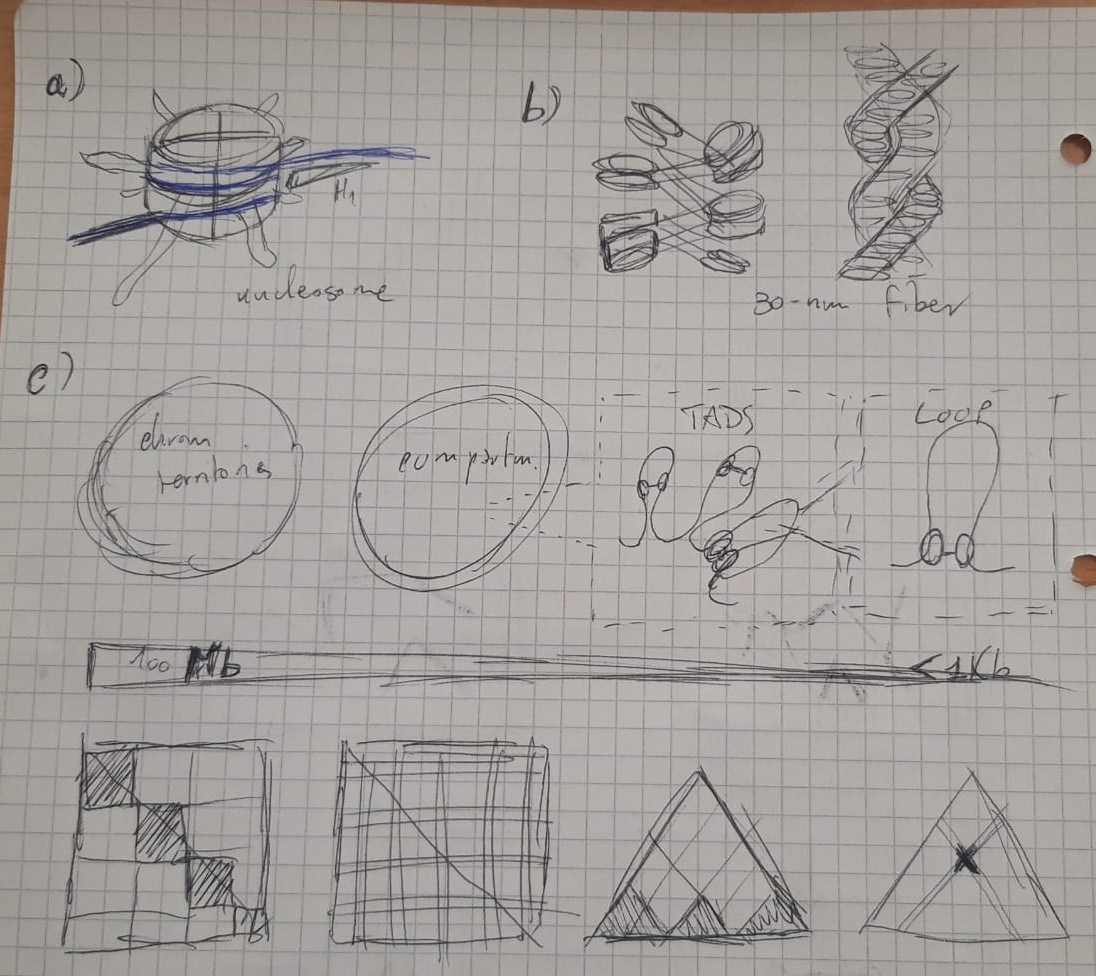
\includegraphics[width=1\textwidth]{chromatin_organization.jpeg}
  \caption{\textbf{Chromatin 3D-organization levels}. Double-strand DNA wraps around a proteic octamer in order to obtain the nucleosome core particle (NCP), which together with linker DNA forms the nucleosome. Nucleosomes are placed along chromatin with a variable spacing, defining the so called "beads-on-a-string" structure. This fiber is then shaped into loops through cohesin complexes; these loops bring into close proximity genes and cis-regulatory elements. The loops are organized into topologically associated domains (TADs) by CTCF, limiting which regions can interact with each other. TADs belong to either chromatin compartment A or B, the former being transcriptionally active, the latter being transcriptionally repressed. Each interphasic chromosome occupies a distinct territory, or area, of the nucleus.}
  \label{fig:chromatin}
\end{figure}

\subsection{Chromatin functions}

Aside from allowing the genetic material to fit into the nucleus, the main role of chromatin is to regulate gene transcription. First of all, nucleosome positioning, histone tails modification and many other factors are all fundamental in defining chromatin accessibility by the transcriptional machinery\cite{chromatinfiber2015, histonemodification2007}. It is in fact possible to define, on a mesoscale level, two \textbf{chromatin states}, those being heterocromatin and eucromatin. The former is a more tightly packed state, meaning that genes located within this region are less transcribed since transcriptional machinery binding is impeded; the latter is a more loosely packed state, favouring gene accessibility and transcription\cite{heterochromatin2020}. Chromatin states and compartments are not necessarily overlapping, even though compartment A tends to be mostly composed of euchromatin and vice versa. Reflecting the role in gene regulation, the chromatin state of a genomic region is not fixed and it can in fact change overtime, for instance by the action of chromatin remodeling complexes\cite{chromatinremodeling2021}. Moreover, the states are associated with different histone modifications which can be added or removed overtime by many enzymes\cite{histonemodifications2020, epigeneticbook2020}.

Another element strongly connected to transcription regulation by chromatin are \textbf{nuclear condensates}, those being areas of the nucleus with an enrichment of molecules linked to some function\cite{condensates2023}. Condensate formation seems to be driven by phase-separation, though the mechanism responsible of selecting which molecules will take part in a specific type of condensate is still unclear\cite{phaseseparation2022}. Condensates can have different sizes and functions; some examples are the nucleolus (for ribosomal RNA transcription), nuclear speckles (for splicing), Cajal bodies (for spliceosomal RNA maturation) and DNA repair foci\cite{condensatetypes2020}. Of particular interest for our discussion are \textbf{transcriptional condensates}, which are smaller scale condensates composed of RNA Pol II, transcription factors and other molecules, whose role is to promote the clustering of cis-regulatory elements, favouring enhancer-promoter interactions\cite{condensatecomposition2018, condensateenhancer2018}. Transcriptional consensates appear to be involved in defining chromatin structure, while at the same time they seem to depend on CTCF and cohesin for the phase-separation process\cite{condensatectcf2022, condensatecohesin2021}. Condensate are also involved in nongenetic functions, which are still being discovered and studied\cite{condensates2023}.

Given the importance of chromatin conformation for gene regulation, its role in organism developement and cell differentiation has been studied in depth\cite{chromatindevelopment2019}, as well as its role in other physiological processes such as X chromosome inactivation\cite{xsilencing2017} and environment response\cite{epigeneticsenvironment2019}. Then, one must take into account that there exist many other processes which, although not directly due to the gene regulation function, are still fundamentaly affected by chromatin organization, among which DNA replication\cite{chromatinreplication2017} and repair\cite{chromatinrepair2017}. Considering this myriad of functions, all of which could be dysregulated leading to pathologies, it becomes evident why improving our understanding of chromatin organization is paramount.

\subsection{Involvement of chromatin in disease}
Considering how complex and highly regulated chromatin conformation is, it is easy to see how its dysregulation can lead to different pathologies. Some examples are reported to show different pathological mechanisms.

The term \textbf{chromatinopathies} refers to rare Mendelian diseases caused by haploinsufficiency in some chromatin regulator gene. When the altered gene pertains transcriptional condensate formation, chromatinopathies manifest mostly with aberrant neurological development and growth abnormalities (either in excess or defect). An example of this type of pathology is Kabuki syndrome\cite{condensates2023}.

Alterations in genes coding for structural proteins can lead to changes in the nuclear mechanical properties and its ability to withstand stress. Mutations in the LMNA gene, coding for the proteins lamin A and C which are fundamental for chromatin organization, have been shown to lead to cardiomyopathies\cite{chromatincardiomyopathy2021}. 

Another mechanism which can lead to altered chromatin conformation are \textbf{structural variants}, those being defined as DNA sequence differences larger than 50 bp from the reference genome\cite{sequencevariations2023}. A common cause of structural variants are inversions. If an inversion happens in proximity of a TAD boundary, this might disrupt its structure, leading to abnormal gene-enhancer interactions (\emph{enhancer hijacking}); this mechanism has been found in both developmental diseases such as polydactyly and brachydactyly\cite{epigeneticlimb2015} as well as different types of both solid and hematopoietic tumors\cite{chromatincancer2022, sequencevariations2023}.

\newpage
\section{Ligation-based methods for the study of chromatin organization}

There exist plenty of methods to study chromatin organization, which can be divided into imaging-based, ligation-based and ligation-free methods. Ligation-based methods stem from one original method, chromosome conformation capture, which has been modified over time to increase resolution and throughput. From the derived methods, Hi-C was the first which allowed to study interactions on a genome-wide scale.

\subsection{Chromosome conformation capture}
Chromosome conformation capture (3C), the original ligation-based method, is a technique which allows to study interactions among genomic regions through \textbf{chromatin crosslinking} and \textbf{proximity ligation}\cite{3coriginal2002}. The main steps of the original protocol are the following:
\begin{itemize}\tightlist
  \item formaldehyde fixation of isolated, intact nuclei. Formaldehyde causes a crosslinking reaction which stabilizes protein-protein and protein-DNA interactions; this means that DNA regions will be in proximity to each other thanks to their protein mediated interactions. 
  \item chromatin digestion through a restriction enzyme (EcoRI).
  \item fragment ligation at very low DNA concentration. In this condition, ligation among DNA fragments crosslinked through proteins is heavily favoured, given that they will always be in proximity of each other.
  \item crosslinking reversion and DNA purification.
  \item quantitative PCR using locus specific primers. Contact frequency among two loci is given by the ratio between the quantity obtained through quantitative PCR on the sample and that obtained using a control.
\end{itemize}
It is important to notice that this is a \textbf{1 vs 1 technique}, meaning that only one pair of loci can be analysed at a time; moreover each comparison requires 2 quantitative PCRs (sample and control) and a pair of locus specific primers, thus requiring some prior knowledge of the target. For these reason the technique is very limited and was modified over time to become 1 vs all (4C\cite{4cprotocol2006}), many vs many (5C\cite{5cprotocol2006}) and then finally all vs all with Hi-C.


\subsection{Hi-C protocol}
Hi-C was the first ligation-based method to allow a \textbf{genome wide} study of chromatin interactions. It differs from the original 3C technique mostly for nucleus lysis using sodium dodecyl sulfate (SDS), the usage of biotin to tag and enrich ligation products and for the usage of \textbf{sequencing} for quantification rather than quantitative PCR\cite{hicoriginal2009}. An optimization of the original Hi-C protocol is in situ Hi-C, whose main difference is that it does not perform nuclear lysis; this reduces the number of ligation events due to random interaction of DNA fragments in solution, while at the same time reducing the reaction volumes and increasing the number of captured interactions\cite{insituhic2014}. The standard in-situ Hi-C protocol, represented in figure \ref{fig:pipeline} (a), can be summarised as follows:

\begin{itemize}\tightlist
  \item DNA crosslinking on intact nuclei
  \item chromatin digestion through a restriction enzyme
  \item filling of the sticky ends at the restriction sites with biotinilated nucleotides
  \item proximity ligation of the now flat and tagged ends
  \item crosslinking reversion and DNA shearing (to 400 bp size)
  \item fragment pulldown using streptavidin beads
  \item elutio and pair-ends sequencing
\end{itemize}
 
Altough in-situ Hi-C is the most common variant of the Hi-C protocol, it is not the only one. Worth of notice is Micro-C, which uses micrococcal nuclease as a restriction enzyme for DNA digestion. This means that all linker DNA is degraded and only interactions among nucleosomes are kept. Given the smaller fragment size, this results in a higher resolution at shorter genomic distances, while long range interactions are poorly captured, making this technique complementary to Hi-C rather than a replacement\cite{microc2015}.

\begin{figure}[ht]
  \centering
  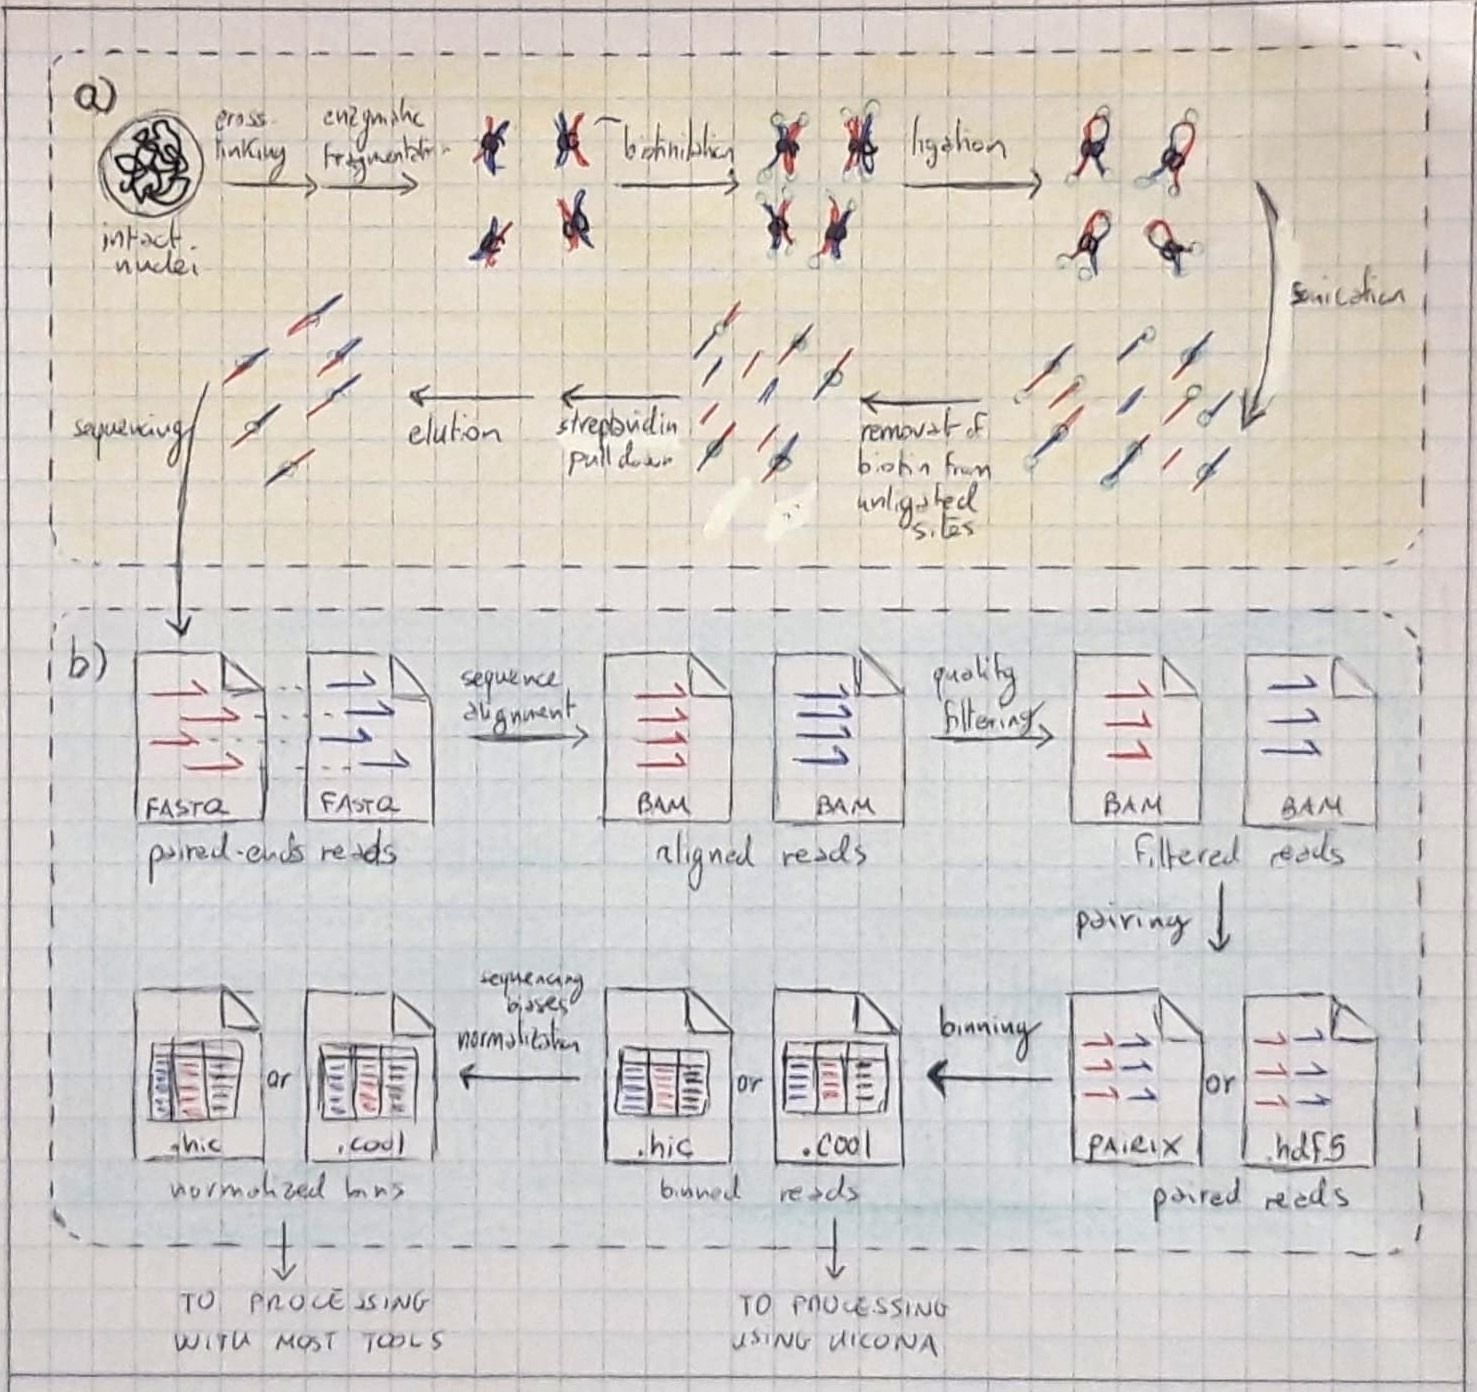
\includegraphics[width=1\textwidth]{hic_pipeline.jpeg}
  \caption{\textbf{Hi-C data generation and analysis workflow}. Steps required to generate Hi-C data files using the in situ Hi-C protocol and the basic sequencing data preprocessing. (a) Main steps of an in situ Hi-C experiment. (b) In-silico steps to generate Hi-C data files starting from the raw paired-ends sequencing reads.}
  \label{fig:pipeline}
\end{figure}

\newpage
\section{Hi-C data storage and analysis}

Handling Hi-C sequencing data is rather challenging for several reasons, both in terms of storage and analysis itself. This type of data requires different processing steps and file formats with respect to standard genomic DNA sequencing, thus requiring specifically designed tools and algorithms. The following subsections will cover the typical steps used to obtain contact matrices strarting from raw sequencing data\cite{hicprocessing2018}; these steps are shown in figure \ref{fig:pipeline} (b). The most common representations and file formats for Hi-C data are also presented.

\subsection{Sequence alignment and binning}
The sequencing step of a Hi-C experiment generally yields some billions of \textbf{paired-end} reads. The fragments from which the reads are derived are chimeric, meaning that they are composed of sequences from regions which are (typically) not genomically contiguous. For this reason it is assumed that the two paired-ends can be mapped independently using standard tools such as bowtie. Still, it is important to notice that, especially for longer reads, the junction among the two interacting genomic regions might fall within one of the paired reads, making the read itself chimeric. \textbf{Chimeric reads} are difficult to map and require apposite strategies which are implemented by Hi-C data specific tools in order to avoid losing a huge amount of information. The aligned reads are then filtered using both standard DNA sequencing criteria, such as base quality and PCR artifacts, as well as Hi-C specific ones, such as self-ligation products, compatibility with undigested chromatin\cite{readfiltering2013} or more elaborate and \emph{ad hoc} ones\cite{complexfiltering2017}.

\textbf{Binning} is the next main step performed; the genome is divided into regions, the bins, and each read is substituted with the bin it falls into. The objective of this procedure is to discretize the signal in order to reduce noise, since it is easier to define the contact frequencies among two regions if they have well defined boundaries (even though this comes with a reduction in resolution).
Although using bins of variable size is an option, fixed-size bins are the more common choice since they are easier to work with. The chosen bin size will affect the resolution of the final contact matrix. The bigger the bin size, the lower the resolution but the more robust the signal; conversely, the smaller the bin size, the higher the resolution but the noisier the signal. Virtually any bin size coul be used, though common sizes span the order of some kilobases (1-10 kb). Bins are assigned a progressive numeric id, from 0 to the number of bins minus 1, to avoid having to refer to them with the entire genomic coordinates they correspond to; sticking to 10 kb resolution, chromosome 1 from base 1 to 10000 would be bin 0, chromosome 1 from base 10001 to 20000 would be bin 1 and so on. After binning, the aligned paired-end reads are thus substituted by pairs of bin ids; it is then possible to count the number of occurrencies (absolute frequency) of each pair, which corresponds to counting how many times the two genomic regions represented by the bins have been found in contact with each other. 

Even though Hi-C has a relatively high throughput, a single experiment, even with very high coverage, rarely yields enough reads for robust analysis in the later steps. For this reason, it is very common to aggregate the reads coming from different biological and technical replicates into a single data file.

\subsection{Contact matrix and ijv table}

The aligned, filtered and binned Hi-C data can be represented either using a contact matrix or using an \emph{ijv} table; these formats are illustrated and compared in figure \ref{fig:contacts} (a).

A \textbf{contact matrix} is a symmetric and sparse matrix, with all the bins the genome has been divided into as both rows and columns. This means that each cell of the matrix represents how many times the bin corresponding to its row has been found in contact with the bin corresponding to its column. A contact matrix is usually displayed using a heatmap, where each cell is represented by a colored square with intensity proportional to the cell value. For this reason each cell of the matrix is also refferred to as \textbf{pixel}. Using a contact matrix it is possible to visualize many chromatin organization levels, as shown in figure \ref{fig:contacts} (b); actually, TADs and compartments were discovered from these heatmaps. Aside from being convenient for visualization purposes, a contact matrix is also convenient to perform row or column-wise operations. For instance, given a certain bin, one can easily obtain the list of interacting bins by looking at the non-zero cells in the corresponding row, or one can compute the number of interactions for that bin by summing the values of all cells in the corresponding row. On the other hand, a contact matrix is not a convenient way to store data. The size of the contact matrix scales quadratically with the number of bins the genome has been divided into; with an itermediate bin size of 10 kb, a contact matrix corresponding to the entire human genome has around $10^{11}$ cells. For this reason a contact matrix can become hard to handle and store into memory, especially as the resolution increases.

The \textbf{\emph{ijv} table} is a format which allows for efficient Hi-C data storage by taking advantage of the properties of the contact matrix. Since the contact matrix is symmetric (the bin contacts are not directional), only the upper triagular part of it (the cells on the main diagonal and those above it) can be stored without losing information. Moreover, since it is a sparse matrix, meaning that most cells have value equal to zero, only the cells with non-zero value can be stored. From these consideration one can define an \emph{ijv} table, also called coordinated list format (COO), as a tabular format where each row contains the two bin ids corresponding to the coordinates of the cell and the value associated to it, and only cells with a value greater than zero are stored. This representation drastically reduces the amount of pixels that need to be stored, and can be converted at any point to the full contact matrix version for visualization. Notice that this format is not well suited for row or column-wise operations, since not all the pixels involving a bin are likely to be contiguous. The pixels are in fact ordered in the same way one would encounter them by going over the upper triangular part of the contact matrix from left to right, from top to bottom; this means that the row bin id will always be smaller than or equal to the column bin id, and that the rows are sorted by row bin id, then by column bin id.

\begin{figure}[ht]
  \centering
  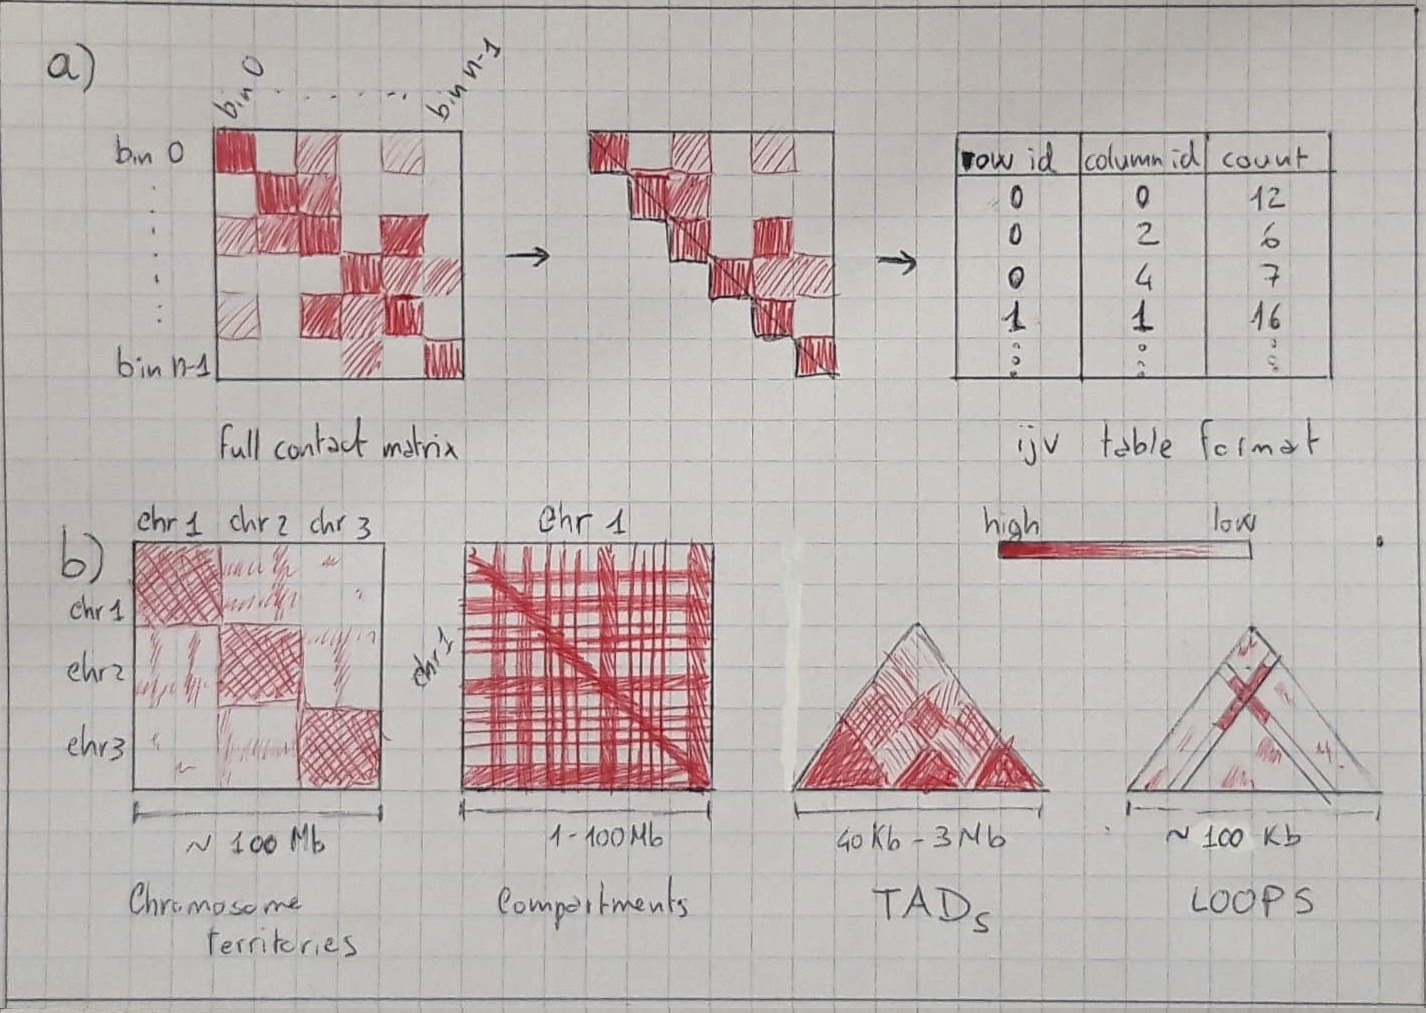
\includegraphics[width=1\textwidth]{contact_matrix.jpeg}
  \caption{\textbf{Contact matrix and ijv table}. (a) Graphical comparison between contact matrix (left) and ijv table (right). (b) Chromatin structures which can be observed through a contact matrix at different scales. From left to right: chromosome territories, compartments, TADs, loops.}
  \label{fig:contacts}
\end{figure}

\subsection{HDF5 and cooler file formats}
An \emph{ijv} table is a very long one dimensional array, that could theoretically be $n^2$ rows long, where $n$ is the number of bins the genome has been divided into. Although the full possible size is never reached, a plain text representation of an \emph{ijv} table would be rather limiting in terms of I/O speed. A better choice is to use a compressed, indexed binary file format. 

The Hierarchical Data Format version 5 (\textbf{HDF5}) is a binary file format mantained by the HDF group\cite{hdfgroup}. A HDF5 file is organized hierachically just like a file system, with nested \textbf{groups} corresponding to folders and \textbf{datasets} corresponding to tables. A dataset is a table with one or more columns, but whose cells all share the same datatype; in order to represent tables with heterogeneous column datatypes, a typical solution is to create the columns as individual datasets, then fetch rows from them simultaneously. Each dataset can be compressed using different algorithms, the default one being gzip. Both groups and tables can be associated with some metadata, divided into \textbf{attributes}, leading the format to be dubbed as self-descriptive. For all these reasons, the HDF5 file format is ideal for the storage and quick retrieval of big, heterogeneous datasets, which led to its usage in several fields, usually with specialized versions for different applications.

One such specialized version is the \textbf{cooler} file format, which was introduced in order to facilitate the storage and retrieval of Hi-C data (or any other type of genomically labeled array)\cite{cooler2020}. A cooler file is therefore a HDF5 with a specific structure, represented in figure \ref{fig:cooler} (a). Each file contains 4 main groups:
\begin{itemize}\tightlist
  \item \emph{bins}, containing ids and genomic coordinates of the bins the genome was divided into.
  \item \emph{pixels}, containing the actual contact matrix in \emph{ijv} form.
  \item \emph{chroms}, containing ids for the chromosomes of the reference genome and their lengths.
  \item \emph{indexes}, containing indexes for the pixels group, for faster pixel retrieval.
\end{itemize}
Each of these groups contains several datasets which represent individual columns of a single table, which is a common practice for HDF5 files as previously mentioned; since the group itself merely acts as a container to group the columns, from here on, the term \textbf{table} will be used to refer to the table obtained by joining the individual datasets present in the group.

Each row in the \textbf{bins table} represents one of the bins the genome has been divided into. For each bin, \texttt{chrom}, \texttt{start} and \texttt{end} positions are always specified (e.i. "\texttt{chr1  10001  20000}"), while any number of columns containing additional bin annotations can be present. In general, the package \emph{cooler}, used to create these files, adds some columns with bin weights for normalization purposes (see next subsection), but any other type of annotation, such as the presence of functional elements (e.i. promoters), can be present. While there is no column reserved for bin ids, the index of the bin in the bin table itself is the bin id; this way it becomes easy to retrieve a certain bin by simply knowing its id.

The \textbf{pixel table} is the \emph{ijv} representation of the contact matrix. Each row has exactly three values, those being \texttt{bin1\_id}, \texttt{bin2\_id} and \texttt{count}, where the first two are the ids of the two interacting bins (row and column bin, respectively), while the third is the raw number of contacts found after binning and counting the aligned paired-ends reads. By referring to the bins via their ids, the pixel table can be drastically simplified, since each bin can be identified using just one column rather than the three necessary to specify the genomic coordinates. At any point, a subset of the pixel table can be converted to the extended form, in which bins are identified by their genomic coordinates, via the process called pixel annotation.

A \texttt{.cool} file contains only one pixels table at one resolution (one bin size). A multiresolution cooler, or \texttt{.mcool} file, is a collection of \texttt{.cool} files referring to the same experiment but at different resolutions. It is itself a single HDF5 file, with a root group called \texttt{resolutions} in which the individual coolers can be found in groups named after the binning resolution, as shown in figure \ref{fig:cooler} (b). It is important to notice that this format is mostly designed for grouping purposes; the different resolutions are completely independent from each other during processing, therefore working on one does not impact the others. Another specialized form of cooler format is the \texttt{.scool} format, which is instead a collection of \texttt{.cool} (or \texttt{.mcool}) files corresponding to different cells and it is thus used for single cell experiments. Its structure is shown in figure \ref{fig:cooler} (c).

\begin{figure}
  \centering
  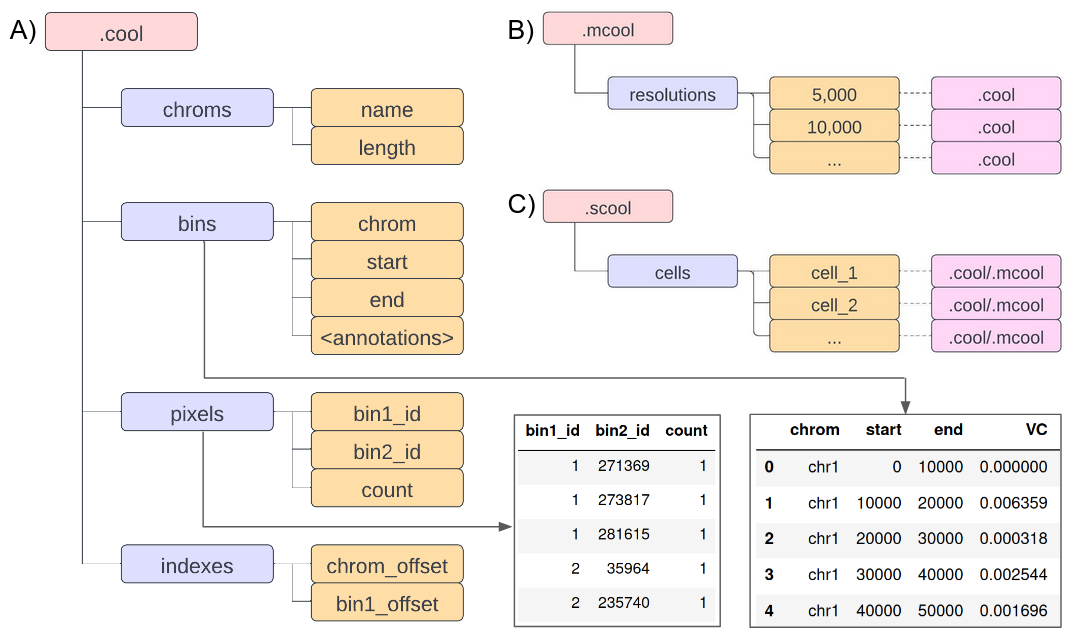
\includegraphics[width=1\textwidth]{cooler_format.png}
  \caption{\textbf{Structure of cooler files and derivates}. Specifics of .cool, .mcool and .scool file formats. (a) .cool file structure, which includes bins, pixels, chromosomes and indexes groups. (b) .mcool file structure, where each group in the resolution one corresponds to a .cool file. (c) .scool file structure, where each group in the cells one corresponds to either a .cool or an .mcool file.}
  \label{fig:cooler}
\end{figure}

\subsection{Sequencing biases normalization strategies}

Different bins have different genomic sequences and properties, leading to different sequencing biases. Several normalizations strategies for systematic biases in Hi-C data exist and none of them seems to be a clear cut winner with respect to the others\cite{normalization2020}. These normalization methods can be divided into explicit and implicit methods. 

\textbf{Explicit methods} are methods which correct for a clearly defined set of systematic biases, such as GC content and mappability. The biases are assumed to be independent from each other; thus, for each bias, a normalization factor is computed for each bin, then the normalization factors are combined to obtain the overall bin normalization factor. It is important to notice though, that this type of technique generally considers the bins homogeneous, which even at a fairly low bin sizes might be seen as a major approximation. For instance, it is obvious that a 5 kb genomic sequence could be divided into areas with very distinct GC content; yet a single GC content normalization factor is applied to all reads falling into the bin, disregarding the fact that a read will never cover the entirety of the bin and it might fall in areas with significantly higher of lower GC content than the average for the bin.

\textbf{Implicit methods} are methods which do not clearly state the systematic biases to correct for. Their assumption is that all systematic biases are recapitulated by sequencing depth, and therefore, making sequencing depth comparable among bins should correct for all of them, whether they are known or not. This in turn equates to assuming that all genomic regions form the same number of interactions and that there is the same number of copies of each region in the genome (no aneuploidies). This is usually achieved through matrix-balancing methods, a class of mathematical algorithms which try to shape a matrix into some constrained form (in this case, comparable bin coverages) while retaining most of the properties of the original matrix. Among matrix-balancing methods, the most common are iterative correction and eigenvector decomposition (ICE)\cite{ice2012} and Knight-Ruiz (KR)\cite{knightruiz2012}, which are also commonly used as weight columns in \texttt{.cool} files. Matrix-balancing methods are individual-sample normalization approaches and they are generally outperformed by cross-sample normalization ones, especially in regards of reproducibility. Still, individual-sample normalization approaches have the major advantage of usually being significantly faster, also considering the fact that one file has to be normalized only once regardless of how many analyses and comparisons will be performed on it. For this reason matrix-balancing methods are the more common ones.

After computing bin normalization factors, be it through explicit or implicit methods, the pixel counts can be normalized by applying (usually by multiplying) the normalization factors of the two bins consituting the pixel. This entails a further assumption, that is that systematic biases as independent across bins.

% \subsection{Hi-C data analysis}

% As stated while discussing chromatin organization, different structures and levels of organization are distinguishable depending on the scale the analysis is being conducted at. For this reason, there exist many tools which study one or many of these different aspects of chromatin conformation, though in general the tools can be classified according to whether they can be used to study compartments, TADs, loops or for visualization\cite{hicprocessing2018}.

\section{Network analysis}

A network is an object describing a set of entities and how they are connected to each other. Networks are a very convenient way of representing complex interactions among any type of entities, and are therefore adopted by many fields, including biology. The mathematical field responsible for the study of networks is graph theory, and for this reason the terms network and graph will be used interchangeably throughout the discussion. In the following subsections, some basic graph theory concepts useful to understand the algorithms presented in the methods chapter, will be introduced. Then, different methods to represent a graph will be briefly compared.
% Then, some of the advantages of network analysis with respect to other mathematical methods will be presented.

\subsection{Graph theory concepts}
A graph is a mathematical object $G$ defined over a set of vertices, or nodes, $V$ and a set of edges $E$, which can therefore be written as $G=(V,E)$. The vertices represent the entities of the graph, while the edges represent the connections among them. Graph order is defined as the number of its nodes ($|V|$), while graph size is defined as the number of its edges ($|E|$).

An edge is a pair of vertices belonging to the graph. If the pairs of vertices are ordered, meaning that $(v_1,v_2)$ and $(v_2, v_1)$ are distinct, the graph is said to be directed; conversely, if the pairs are not ordered, meaning that $(v_1,v_2) \equiv (v_2, v_1)$, the graph is said to be undirected. Moreover, if a weight is assigned to each edge, the graph is called weighted, else it is called unweighted. The different types of graph are shown in figure \ref{fig:networks} (a).

The degree of a node is the number of incident edges, meaning the number of edges touching it; if the graph is directed, one can distinguish between out-degree and in-degree, those being the number of times the node appears as first or second element in the ordered pairs, respectively. The neighbours of a node are the nodes which are directly connected to it by an edge (e.i. both nodes are incident to the same edge); the set of neighbours of a node is collectively referred to as neighbourhood. In a weighted graph, node strenght is the sum of the weights of all incident edges. 

Graph density is a measure of how interconnected the nodes of the graph are on a global scale; graph density is defined as the number of edges present in the graph over the number of possible edges for that graph, which is $|V|(|V|-1)/2$ in the undirected case, $|V|(|V|-1)$ in the directed one. 
% Connected components?

\subsection{Graph representations} 

Aside from the standard graphical representation using lines and dots, a network has three other major representation methods: edge list, adjacency matrix and adjacency list. These are shown in figure \ref{fig:networks} (b).

A network can be represented using an \textbf{edge list}, which corresponds to listing all edges which do exist in the network, ideally in an ordered manner. This representation is memory efficient, since all edges are listed only once, but it is not very convenient for searching specific edges.

An \textbf{adjacency matrix} is a matrix with all nodes of the graph as both rows and columns. If the edge individuated by a set of coordinates (e.i. a pair of nodes) exists, the corrisponding cell will contain the edge value (edge weight in the weighted case, 1 in the unweighted one); if it is not present, the cell will contain zero. Notice that in the case of an undirected graph, the matrix is symmetric with respect to the main diagonal. This representation is not memory efficient, especially for sparse graphs, since it always stores $|V|^2$ values, but it is quite fast to retrieve all node neighbours and in general perform operations. 

In the \textbf{adjacency list} representation, a list containing all neighbours is associated to each node. This representation is as memory efficient as the edge list when used for directed graphs, since all edges are listed only once; in case of an undirected graph, this representation is slightly less memory efficient, since each edge is present in the adjacency list of both incident nodes, therefore requiring to store $2|V|$ values. This representation is convenient in order to retrieve node neighbours, though not quite as convenient for other types of operations. 

\begin{figure}[hb]
  \centering
  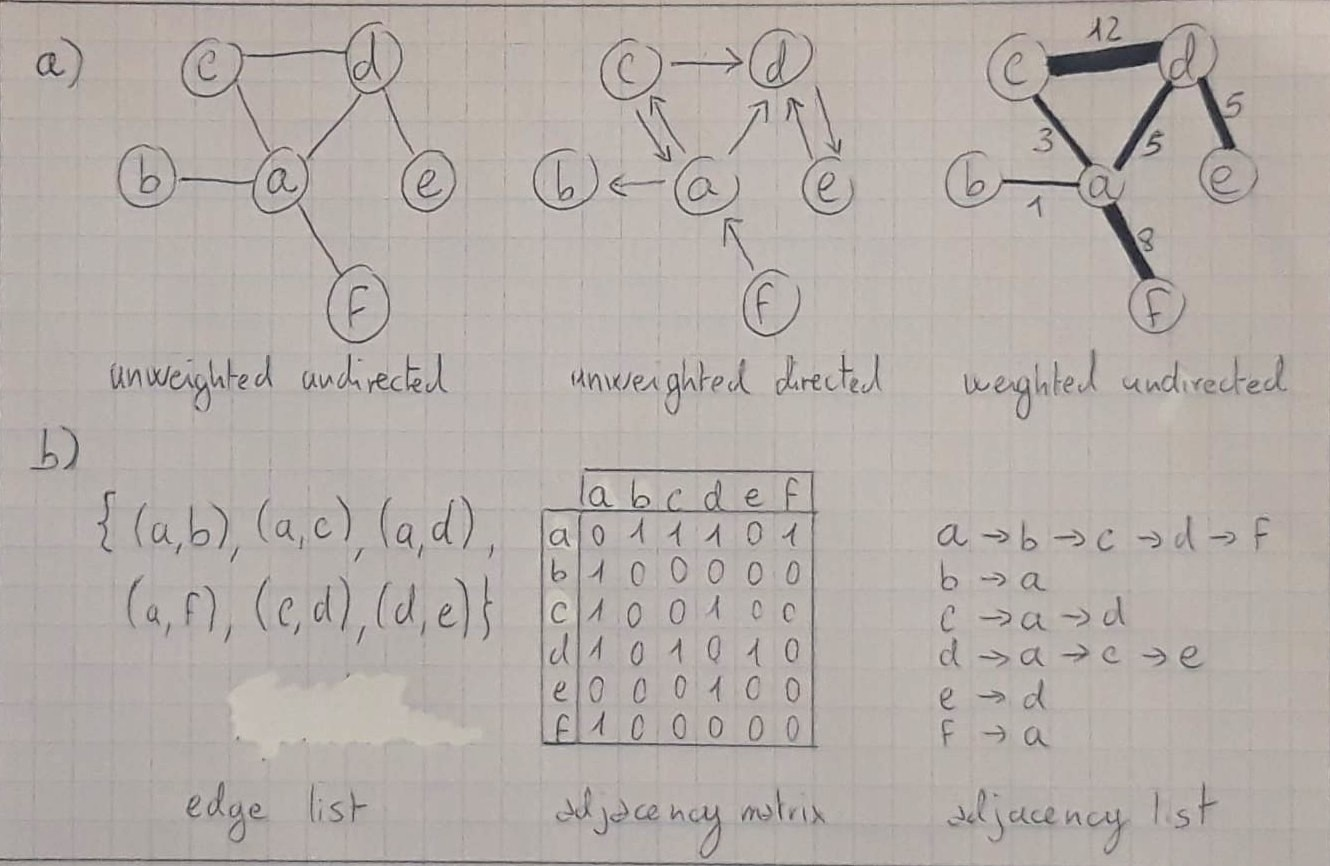
\includegraphics[width=0.9\textwidth]{networks.jpeg}
  \caption{\textbf{Graph features and representations}. a) Different types of networks. Considering the unweighted undirected graph, we can say that it has both order and size equal to 6. Taking as an example node $a$, in the undirected cases both in-degree and out-degree are equal to 4, while in the directed case its in-degree is 2 while its out-degree is 3. The neighbourhood of node $a$ in the unweighted undirected graph is the set of nodes $\{b,c,d,f\}$. In the weighted case, the strength of node $a$ is given by the sum of its incident edges, which equates to 17. b) Different ways of representing a network. From left to right, edge list, adjacency matrix and adjacency list representation of the unweighted undirected graph from point \emph{a} of this image.}
  \label{fig:networks}
\end{figure}

